%\documentclass[draft,grl]{AGUTeX}
\documentclass[twocolumn,grl]{AGUTeX}
\usepackage{mathptmx}
% \usepackage{lineno}
% \linenumbers*[1]

%  To add line numbers to lines with equations:
%  \begin{linenomath*}
%  \begin{equation}
%  \end{equation}
%  \end{linenomath*}

%  Uncomment the following command to include .eps files
%  (comment out this line for draft format):
%\usepackage[dvips]{graphicx}
\usepackage[pdftex]{graphicx}
%\setkeys{Gin}{draft=false}

\authorrunninghead{STYRON AND HETLAND}
\titlerunninghead{LANF EARTHQUAKE LIKELIHOOD}

\authoraddr{Corresponding author: Richard H. Styron,
Department of Earth and Environmental Sciences, University of
Michigan, 2534 CC Little Bldg., 1100 N. University Ave., 
Ann Arbor, MI 48104, USA (richard.h.styron@gmail.com)}

\begin{document}
\title{Likelihood of observing an earthquake on a low-angle normal fault}

\authors{Richard H. Styron \altaffilmark{1}
and Eric A. Hetland \altaffilmark{1}}

\altaffiltext{1}{Department of Earth and Environmental Sciences, University of
Michigan, Ann Arbor, Michigan, USA.}

\begin{abstract}
Lorem ipsum dolor sit amet, consectetur adipiscing elit. Morbi non felis egestas, pharetra eros sed, euismod leo. Donec et hendrerit lorem, quis facilisis urna. Phasellus vel dolor quis dui viverra blandit. Interdum et malesuada fames ac ante ipsum primis in faucibus. In neque lacus, viverra et aliquam id, luctus non lectus. Suspendisse accumsan ipsum sem, sit amet commodo augue dignissim ac. Suspendisse mi sapien, malesuada non enim sed, vehicula tincidunt nisl. In varius, felis ut sagittis porta, sem nisi pulvinar velit, a malesuada purus nulla vitae eros. Phasellus accumsan et lacus vel eleifend. Mauris leo augue, aliquet a nunc sed, blandit faucibus augue. In hac habitasse platea dictumst. Proin in ultrices metus. Donec consequat porta aliquam. Praesent ligula nibh, congue nec porttitor sed, elementum id nibh. Etiam tristique egestas augue. 
\end{abstract}

\begin{article}

\section{Introduction}
Low-angle normal faults (LANFs), with dips less than 30$^\circ$, are well described in the geologic record. They are hypothesized to have an important role in accommodating large-magnitude continental extension \citep{howard1987crustal} and crustal thinning \citep{lister1986detachment}, and their recognition has been one of the most important developments in tectonics over the past several decades \citep{wernicke2009detachment}. However, despite widespread field observations of inactive LANFs and their central role in modern extensional tectonic theory, they remain enigmatic and contentious structures. This is for two reasons: because brittle faulting on LANFs is in apparent conflict with standard Andersonian rock mechanical theory as typically applied to the upper crust \citep{axen2004lanfmech}, and because observations of active faulting on LANFs is sparse and at times ambiguous \citep{wernicke1995seis}. A considerable amount of research has been performed to address the former concern, reconciling LANF slip with rock mechanics. The latter issue, the paucity of observations, has inhibited hypothesis testing of LANF fault theory, and has also contributed to a mode of thought where the absence of evidence for LANF seismicity is taken as evidence of its absence \citep{jackson1987, collettinisibson2001}. Alternately, the lack of observed seismic slip on a continental LANF may be explained by the rarity of seismicity and the small number of potential active structures.

In this work, we choose to directly address the question of whether the lack of observed seismicity may be interpreted as an indication that LANFs may not slip seismically, or is better explained as an effect of the small number of active LANFs, which are seismogenic.  We do this by calculating the likelihood of observing a moderate to large earthquake on a LANF over different time windows, assuming that all continental LANFs described in the literature are seismically active at their surface dip angles and display typical seismic behavior.

\subsection{LANF Slip, Mohr-Coulomb failure theory, and Seismicity}
Areas of the crust undergoing active extension are generally assumed to have a subvertical maximum compressive stress.  Mohr-Coulomb theory as applied to the crust predicts that a fault with a typical coefficient of friction for rocks (0.6--0.8) should lock up if it is oriented at an angle greater than 60$^\circ$, and new, optimally oriented faults should form \citep{sibson1985}.  Therefore, for normal faults with dips less than 30$^\circ$, either much lower fault friction or elevated pore fluid pressure is required for these faults to slip.

Evidence for seismic slip on LANFs is sparse.  
Mauris eget sodales orci. Morbi porttitor sit amet arcu sit amet pharetra. Phasellus mattis vulputate elit ut commodo. Suspendisse rhoncus vestibulum urna, non dictum metus. Donec sed rhoncus magna. Vivamus at auctor massa, at eleifend velit. Phasellus ullamcorper a nulla non euismod. Nulla ante elit, egestas a luctus sit amet, lacinia nec felis. Sed condimentum, nunc a vehicula ullamcorper, augue urna cursus tortor, sit amet auctor tortor tellus eu elit. Nunc ut bibendum enim. Curabitur volutpat blandit ullamcorper. Nam mollis quam quis viverra auctor. Aenean posuere lacus quis sapien elementum, vel rhoncus nunc dignissim. Nullam in risus nisi. Morbi sollicitudin velit et lacus interdum, non dictum libero suscipit. Mauris eleifend dui ac tincidunt pharetra. 

\section{Potentially Active LANFs}

Over the past decade or so, many field studies have found evidence for LANF activity in orogens throughout the world. These studies typically find arrays of Quaternary normal fault scarps on the fault traces and/or in the hanging walls of mapped or inferred low-angle detachment faults \citep [e.g.,][]{axen1999baja}. Some studies also have bedrock thermochronology data from the exhumed footwalls of the detachments that is suggestive of ongoing rapid exhumation \citep [e.g.,][]{sundell2013lunggar}, although this data does not preclude a recent cessation of faulting. In some cases, additional evidence for LANF activity comes from geophysical data such as GPS geodesy \citep [e.g.,][]{hreinsdottir2009altotib} and seismic waves \citep [e.g.,][]{doser1987ancash}.

We have compiled all potentially active LANFs with known subareal fault traces from a thorough review of the literature; there are twenty total (Figure~\ref{fig:lanf_map}).  About half are in Tibet, consistent with hypotheses that LANFs and metamorphic core complexes form in areas of hot, thick crust \citep [e.g.,][]{buck1991mcc}.  The rest are distributed through other areas of active continental extension: the North American Basin and Range, the Malay Archipelago, Turkey, Italy, and Peru. Several of the most-commonly cited candidates for seismically active LANFs were not included because they do not have a clearly-defined, mappable fault trace, which is necessary for our calculations.  These include the submarine core complexes in the Woodlark Basin \citep{abers2001}, the fault responsible for the 1995 Aigion, Greece earthquake \citep{bernard1997} and other potential LANFs underneath the Gulf of Corinth, and the fault responsible for the 1952 Ancash, Peru earthquake \citep{doser1987ancash}.

The faults compiled here are all in well-known areas of active extension.  Though the fault traces of many LANFs considered here are obscured by vegetation or agriculture, others display large fault scarps in Quaternary sediments, particularly those in the dry climates of Tibet \citep[e.g.,][]{styron2013slr, kapp2005nqtl} and the western US \citep[e.g.,][]{axen1999baja, hayman2003dv}, which are commonly interpreted as evidence for seismic slip.% \citep[e.g.,][]{\  }.  


\begin{figure*}
\noindent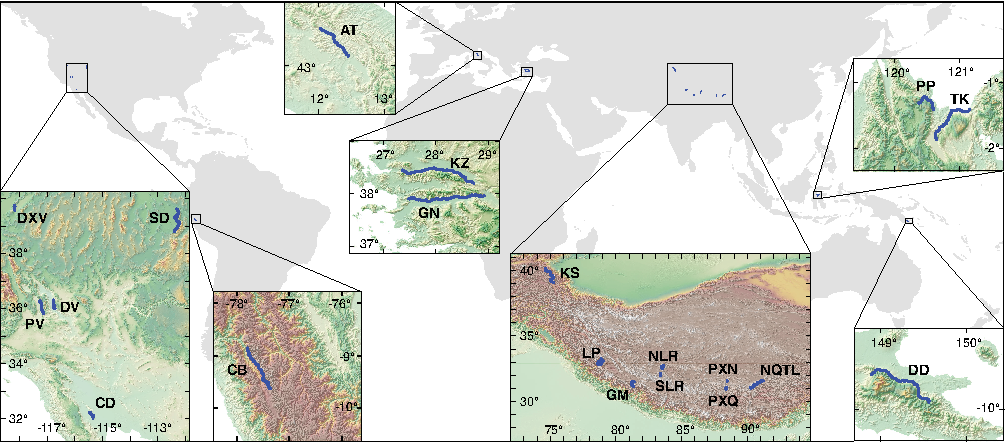
\includegraphics[width=40pc]{./figures/active_lanfs_map_insets.pdf}
\caption{Map of known, potentially active continental LANFs (blue lines), with insets showing the physiographic context of the faults.  DXV=Dixie Valley fault.  PV=Panamint Valley fault.  DV=Death Valley fault.  CD=Ca\~nada David detachment.  SD=Sevier Desert detachment.  CB=Cordillera Blanca detachment.  AT=Alto-Tiberina fault.  KZ=Kuzey detachment.  GN=Guney detachment.  KS=Kongur Shan fault.  LP=Leo Pargil detachment.  GM=Gurla Mandhata detachment. NLR=North Lunggar detachment.  SLR=South Lunggar detachment.  PXN=Pum Qu--Xainza north fault.  PXQ=Pum Qu--Xainza Qingdu fault.  NQTL=Nyainqentanglha detachment.  PP=Papangeo detachment.  TK=Tokorondo detachment.  DD=Dayman Dome.}
\label{fig:lanf_map}
\end{figure*}

We have then mapped the approximate fault traces into a GIS file (available at https://github.com/cossatot/LANF\_gis), with metadata such as slip rate and source. We then have estimated the probability of observing an earthquake above a given magnitude for each fault individually over some time window, and then calculated the probability of observing a significant earthquake on any of the faults over that same time window.

\section{Likelihood of observing a LANF event}
\subsection{Rupture Likelihood on Individual LANFs}
To estimate the likelihood of observing a significant earthquake on an individual LANF over some contiguous time window of length $t$ (in years), we perform a Monte Carlo simulation in which we create 2000 synthetic time series of earthquakes, with unique values for fault geometry and slip rate for each time series. Then, for each time series we calculate the fraction of unique time windows of length $t$ in which an earthquake as large or larger than a given magnitude occurs.  We take this value as the probability of observing an earthquake greater than or equal to moment magnitude \emph{M} in time $t$, which we will refer to in the general sense as $P(M,t)$.

The geometry for each fault is estimated based on the length of the fault trace, the dip of the fault, and the estimated seismogenic thickness or fault locking depth in the area.  The fault is treated as planar for simplicity of calculations, even though the exposed footwalls of many detachment faults are highly corrugated.  We determine the fault length by measuring the approximate length of the mapped fault trace perpendicular to the assumed extension direction; for faults that change dip significantly along strike (e.g., the Dixie Valley fault), we only consider the low-angle segments of the fault.  Values for the dip are taken from the literature in most cases, and measured from SRTM data otherwise; in all cases, a range of values is considered.  The seismogenic thickness or fault locking depth is assumed to be 10 km in the absence of other evidence (such as a geodetic study, \citep [e.g.,][]{hreinsdottir2009altotib}).

Slip rates are similarly gathered from the literature if possible, or given broad ranges if not (e.g., 1--10 mm yr$^{-1}$).  In the Monte Carlo simulation, samples for slip rate and dip are drawn from uniform distributions defined by the maximum and minimum values.  Based on field observations, some faults have dip ranges that go above 30$^\circ$; this study only considers slip on faults shallower than this, so for these faults, dip values are sampled from the minimum to 30$^\circ$ and the resulting probabilities are then multiplied by the fraction of the dip range that is under 30$^\circ$.

Each earthquake sequence is generated by randomly sampling 50,000 events from a tapered Gutenberg-Richter distribution with corner magnitude $M_c = 7.64$ and $\beta = 0.65$ (from values estimated by \citet{birdkagan2004f_m} for continental rifts) using an inverse transform sampling algorithm.  The samples are taken from an interval $M = [5.0, \, M_{max}]$, where $M_{max}$ is calculated as the moment magnitude $M$ resulting from fault slip $D$ = 15 m over a fault of length $L$ cutting through a seismogenic thickness $z$ at dip $\delta$, given the relations 

\begin{equation}
 M_o = \mu L z D \,/ \, \sin \delta 
 \end{equation}

and

\begin{equation}
M = 2/3 \; \log_{10} (M_o) - C 
\end{equation}
where $C = 6 $ and shear modulus $\mu = 30$ GPa, and $M_o$ is the seismic moment.  Sensitivity tests (see Supplementary Materials) show that the results are only slightly affected by the frequency-magnitude distribution: differences between results using this distribution and a `characteristic' distribution with an enhanced probability of earthquakes around $M$ 6 are well below the variability created by uncertainty in fault dip and slip rate.  

Then, a time series of strain accumulation and release for each earthquake sequence is created, with one value per year.  This is constructed by separating each earthquake from the previous one with a set of zeros (representing no significant earthquakes for those years) where the number of zero years before an event corresponds to the length of an interseismic interval necessary to accumulate all the slip released in that event, given the fault dimensions and slip rate for that time series. Then, the likelihood of observing a significant earthquake is calculated as described above.

\begin{figure}[ht!]
\noindent\includegraphics[width=20pc]{./figures/kongur_all_probs.pdf}
\caption{\textbf{a:} Probabilities of observing an earthquake greater than or equal to a given moment magnitude \emph{M} over a given observation window on the Kongur Shan fault (Tibet). \textbf{b:} Probabilities of observing an earthquake greater than or equal to a given moment magnitude \emph{M} over a given observation window on all studied LANFs. }
\label{fig:kongur_all_probs}
\end{figure}

As an example, the results for the Kongur Shan fault are shown in Figure~\ref{fig:kongur_all_probs} a.  The results show that it is unlikely that any earthquake above \emph{M} 5.0 will be observed over time scales up to a century. 


\subsection{Probability on All LANFs}
To calculate the probability of observing an earthquake over the time window on any of the LANFs studied, we first assume that seismicity on each fault is independent and uncorrelated from seismicity on all other faults. This assumption is likely true for most faults, but may not be true for some proximal faults (such as the North and South Lunggar detachments, or the Papangeo and Tokorondo detachments), though it is hard to determine how these faults may interact.  We determine the probability for each time window and minimum magnitude with the equation
\begin{equation}
p_{AT \, or \, LP\, \ldots \, or \, DV} = 1 - (q_{AT} \cdot q_{LP} \cdot \ldots \, \cdot q_{DV})
\end{equation}
where $p_{AT}$ is the probability of observing an earthquake on a single LANF (the Alto-Tiberina fault), and $q_{AT} = 1 - p_{AT}$.

The results of this calculation are shown in Figure~\ref{fig:kongur_all_probs} b.  Unlike the results from a single fault, the results from all faults show that it is likely that a significant earthquake on a LANF would be observed over an observation period of even a handful of years.  If we take \emph{M} 6.0 as the lowest magnitude for which modern, global earthquake catalogs are complete [e.g., ref], and 40 years as the length of those catalogs, then the probability of seeing a significant LANF event is about 0.65.

Here we need a better introduction to the next section.

\subsection{Possible Effect of Inactive Faults}
Of the faults considered here, several have received little to no field study, and others have generated conflict in the literature over whether they are active.  It is possible that these faults spuriously affect the results, raising $P(M,t)$.  To test this, we re-run the final calculations, disregarding the Tokorondo and Papangeo detachments (as they have received no modern field study and do not have clear Quaternary fault scarps in Google Earth imagery), and the Kuzey and Guney detachments, as evidence exists that they are inactive [e.g., refs, G. Axen, personal communication].  Because the smaller faults with lower slip rates do not significantly impact the results (see Supplementary Materials), we do not leave out other poorly-studied or contested faults.
	
The results from the calculations without these faults are shown in Figure~\ref{fig:all_probs_no_maybes} a. The probabilities for the reference  


\begin{figure}%[t!]
\noindent\includegraphics[width=20pc]{./figures/all_M_no_maybes.pdf}
\caption{\textbf{a:} Probabilities of observing an earthquake greater than or equal to a given moment magnitude \emph{M} over a given observation window on the all faults except those in Turkey and Sulawesi. \textbf{b:} Component of total probabilities contributed by the Turkey and Sulawesi faults.}
\label{fig:all_probs_no_maybes}
\end{figure}


\section{Discussion and conclusions}

The results of this study yield twenty potentially active LANFs, and show a moderate likelihood of observing a $\ge M$6.0 event on any of the LANFs in several decades of observation.
This compilation potentially active LANFs shows that they are fairly uncommon structures, yet they may still be found in areas of active extension. The compilation may serve as a point of comparison for different characteristics of active normal faults or LANF geometry, or as a reference for any further related study.

Our statistical modeling results indicate a 50--70\% chance of observing a moderate to large earthquake on a LANF over the 40 or so years of global, automated earthquake detection, assuming that all faults here are seismically active at their surface dip angles.  This likelihood range is not sufficient to reject hypotheses of LANF seismicity or aseismicity. However, these results do provide a quantitative probabilistic context for interpretations of the lack of well-documented continental LANF events.  
For example, these probabilities indicate that it cannot be taken for granted that a significant earthquake should be observed over the `catalog period' of about 40 years. Therefore, results and conclusions of studies analyzing the dip distribution of earthquakes on continental normal faults \citep{jackson1987, collettinisibson2001} should be interpreted in this context.  Similarly, mechanisms such as aseismic creep \citep [e.g.,][]{collettini2011lanfmech, hreinsdottir2009altotib}, isostatic flexure \citep[e.g.,][] {wernickeaxen1988rolling}, or extremely long seismic recurrence intervals \citep{wernicke1995seis} need not be invoked to explain the lack of observed seismicity, though these mechanisms may indeed be valid or well supported by other observations.

It should also be noted that this study gives the \emph{maximum} probability of observing a LANF earthquake given that these are the only active continental LANFs.  Some of these faults may be inactive, such as those in Turkey and Sulawesi; though given that a considerable number of the faults here have been first described in the past 10-15 years, it is also likely that more potentially active LANFs will be discovered in the future.  Many of these faults may have steeper dips in the seismogenic crust, such as the Ca\~nada David detachment in Mexico \citep{fletcherspelz2009}.  Some of these may also be aseismic; the Alto-Tiberina fault appears to be creeping for much of its down-dip extent \citep{hreinsdottir2009altotib}, and the neighboring Zuccale inactive LANF has fault gouge suggestive of creep \citep{collettiniholdsworth2004}.  


\begin{acknowledgements}
We thank Jon Spencer for a stimulating discussion that became the impetus for this study.
\end{acknowledgements}

% put bib here
\begin{thebibliography}{23}
\providecommand{\natexlab}[1]{#1}
\expandafter\ifx\csname urlstyle\endcsname\relax
  \providecommand{\doi}[1]{doi:\discretionary{}{}{}#1}\else
  \providecommand{\doi}{doi:\discretionary{}{}{}\begingroup
  \urlstyle{rm}\Url}\fi

\bibitem[{\textit{Abers}(2001)}]{abers2001}
Abers, G.~A. (2001), Evidence for seismogenic normal faults at shallow dips in
  continental rifts, \textit{Geological Society, London, Special Publications},
  \textit{187}(1), 305--318.

\bibitem[{\textit{Axen}(2004)}]{axen2004lanfmech}
Axen, G.~J. (2004), Mechanics of low-angle normal faults, in \textit{Rheology
  and Deformation of the Lithosphere at Continental Margins}, edited by G.~D.
  Karner et~al., pp. 46--91, Columbia Univ. Press, New York.

\bibitem[{\textit{Axen et~al.}(1999)\textit{Axen, Fletcher, Cowgill, Murphy,
  Kapp, MacMillan, Ramos-Vel{\'a}zquez, and Aranda-G{\'o}mez}}]{axen1999baja}
Axen, G.~J., J.~M. Fletcher, E.~Cowgill, M.~Murphy, P.~Kapp, I.~MacMillan,
  E.~Ramos-Vel{\'a}zquez, and J.~Aranda-G{\'o}mez (1999), Range-front fault
  scarps of the sierra el mayor, baja california: Formed above an active
  low-angle normal fault?, \textit{Geology}, \textit{27}(3), 247--250.

\bibitem[{\textit{Bernard et~al.}(1997)\textit{Bernard, Briole, Meyer,
  Lyon-Caen, Gomez, Tiberi, Berge, Cattin, Hatzfeld, Lachet
  et~al.}}]{bernard1997}
Bernard, P., P.~Briole, B.~Meyer, H.~Lyon-Caen, J.-M. Gomez, C.~Tiberi,
  C.~Berge, R.~Cattin, D.~Hatzfeld, C.~Lachet, et~al. (1997), The ms= 6.2, june
  15, 1995 aigion earthquake (greece): evidence for low angle normal faulting
  in the corinth rift, \textit{Journal of Seismology}, \textit{1}(2), 131--150.

\bibitem[{\textit{Bird and Kagan}(2004)}]{birdkagan2004f_m}
Bird, P., and Y.~Y. Kagan (2004), Plate-tectonic analysis of shallow
  seismicity: Apparent boundary width, beta, corner magnitude, coupled
  lithosphere thickness, and coupling in seven tectonic settings,
  \textit{Bulletin of the Seismological Society of America}, \textit{94}(6),
  2380--2399.

\bibitem[{\textit{Buck}(1991)}]{buck1991mcc}
Buck, W.~R. (1991), Modes of continental lithospheric extension,
  \textit{Journal of Geophysical Research: Solid Earth (1978--2012)},
  \textit{96}(B12), 20,161--20,178.

\bibitem[{\textit{Collettini}(2011)}]{collettini2011lanfmech}
Collettini, C. (2011), The mechanical paradox of low-angle normal faults:
  Current understanding and open questions, \textit{Tectonophysics},
  \textit{510}(3), 253--268.

\bibitem[{\textit{Collettini and Holdsworth}(2004)}]{collettiniholdsworth2004}
Collettini, C., and R.~Holdsworth (2004), Fault zone weakening and character of
  slip along low-angle normal faults: insights from the zuccale fault, elba,
  italy, \textit{Journal of the Geological Society}, \textit{161}(6),
  1039--1051.

\bibitem[{\textit{Collettini and Sibson}(2001)}]{collettinisibson2001}
Collettini, C., and R.~H. Sibson (2001), Normal faults, normal friction?,
  \textit{Geology}, \textit{29}(10), 927--930.

\bibitem[{\textit{Doser}(1987)}]{doser1987ancash}
Doser, D.~I. (1987), The ancash, peru, earthquake of 1946 november 10: Evidence
  for low-angle normal faulting in the high andes of northern peru,
  \textit{Geophysical Journal of the Royal Astronomical Society},
  \textit{91}(1), 57--71.

\bibitem[{\textit{Fletcher and Spelz}(2009)}]{fletcherspelz2009}
Fletcher, J.~M., and R.~M. Spelz (2009), Patterns of quaternary deformation and
  rupture propagation associated with an active low-angle normal fault, laguna
  salada, mexico: Evidence of a rolling hinge?, \textit{Geosphere},
  \textit{5}(4), 385--407.

\bibitem[{\textit{Hayman et~al.}(2003)\textit{Hayman, Knott, Cowan, Nemser, and
  Sarna-Wojcicki}}]{hayman2003dv}
Hayman, N.~W., J.~R. Knott, D.~S. Cowan, E.~Nemser, and A.~M. Sarna-Wojcicki
  (2003), Quaternary low-angle slip on detachment faults in death valley,
  california, \textit{Geology}, \textit{31}(4), 343--346.

\bibitem[{\textit{Howard and John}(1987)}]{howard1987crustal}
Howard, K.~A., and B.~E. John (1987), Crustal extension along a rooted system
  of imbricate low-angle faults: {Colorado River} extensional corridor,
  {California} and {Arizona}, \textit{Geological Society, London, Special
  Publications}, \textit{28}(1), 299--311.

\bibitem[{\textit{Hreinsd{\'o}ttir and
  Bennett}(2009)}]{hreinsdottir2009altotib}
Hreinsd{\'o}ttir, S., and R.~A. Bennett (2009), Active aseismic creep on the
  alto tiberina low-angle normal fault, italy, \textit{Geology},
  \textit{37}(8), 683--686.

\bibitem[{\textit{Jackson}(1987)}]{jackson1987}
Jackson, J. (1987), Active normal faulting and crustal extension,
  \textit{Geological Society, London, Special Publications}, \textit{28}(1),
  3--17.

\bibitem[{\textit{Kapp et~al.}(2005)\textit{Kapp, Harrison, Kapp, Grove,
  Lovera, and Lin}}]{kapp2005nqtl}
Kapp, J.~L., T.~M. Harrison, P.~Kapp, M.~Grove, O.~M. Lovera, and D.~Lin
  (2005), Nyainqentanglha shan: a window into the tectonic, thermal, and
  geochemical evolution of the lhasa block, southern tibet, \textit{Journal of
  Geophysical Research: Solid Earth (1978--2012)}, \textit{110}(B8).

\bibitem[{\textit{Lister et~al.}(1986)\textit{Lister, Etheridge, and
  Symonds}}]{lister1986detachment}
Lister, G., M.~Etheridge, and P.~Symonds (1986), Detachment faulting and the
  evolution of passive continental margins, \textit{Geology}, \textit{14}(3),
  246--250.

\bibitem[{\textit{Sibson}(1985)}]{sibson1985}
Sibson, R.~H. (1985), A note on fault reactivation, \textit{Journal of
  Structural Geology}, \textit{7}(6), 751--754.

\bibitem[{\textit{Styron et~al.}(2013)\textit{Styron, Taylor, Sundell, Stockli,
  Oalmann, M{\"o}ller, McCallister, Liu, and Ding}}]{styron2013slr}
Styron, R.~H., M.~H. Taylor, K.~E. Sundell, D.~F. Stockli, J.~A. Oalmann,
  A.~M{\"o}ller, A.~T. McCallister, D.~Liu, and L.~Ding (2013), Miocene
  initiation and acceleration of extension in the south lunggar rift, western
  tibet: Evolution of an active detachment system from structural mapping and
  (u-th)/he thermochronology, \textit{Tectonics}.

\bibitem[{\textit{Sundell et~al.}(2013)\textit{Sundell, Taylor, Styron,
  Stockli, Kapp, Hager, Liu, and Ding}}]{sundell2013lunggar}
Sundell, K.~E., M.~H. Taylor, R.~H. Styron, D.~F. Stockli, P.~Kapp, C.~Hager,
  D.~Liu, and L.~Ding (2013), Evidence for constriction and pliocene
  acceleration of east-west extension in the north lunggar rift region of west
  central tibet, \textit{Tectonics}, in press.

\bibitem[{\textit{Wernicke}(1995)}]{wernicke1995seis}
Wernicke, B. (1995), Low-angle normal faults and seismicity: A review,
  \textit{Journal of Geophysical Research}, \textit{100}(B10), 20,159--20.

\bibitem[{\textit{Wernicke}(2009)}]{wernicke2009detachment}
Wernicke, B. (2009), The detachment era (1977--1982) and its role in
  revolutionizing continental tectonics, \textit{Geological Society, London,
  Special Publications}, \textit{321}(1), 1--8.

\bibitem[{\textit{Wernicke and Axen}(1988)}]{wernickeaxen1988rolling}
Wernicke, B., and G.~J. Axen (1988), On the role of isostasy in the evolution
  of normal fault systems, \textit{Geology}, \textit{16}(9), 848--851.

\end{thebibliography}



\end{article}

%put figures here for submission

%\bibliographystyle{agufull08}
%\bibliography{styron_hetland_lanf}

\end{document}


